\documentclass[a4paper,10pt]{amsbook}

\usepackage[T1]{fontenc}
\usepackage{lmodern}
\usepackage[utf8x]{inputenc}
\usepackage[italian]{babel}

\usepackage{amsmath}
\usepackage{amssymb}
\usepackage{amsthm}
\usepackage{xfrac}
\usepackage[all]{xy}
\usepackage{graphicx}
\usepackage{algorithm}
\usepackage[noend]{algpseudocode}
%\usepackage{fullpage}
\usepackage{hyperref}
\usepackage{chngcntr}


%\setlength{\parindent}{0in}

\newcounter{counter1}

\theoremstyle{plain}
\newtheorem{myteo}[counter1]{Teorema}
\newtheorem{mylem}[counter1]{Lemma}
\newtheorem{mypro}[counter1]{Proposizione}
\newtheorem{mycor}[counter1]{Corollario}
\newtheorem*{myteo*}{Teorema}
\newtheorem*{mylem*}{Lemma}
\newtheorem*{mypro*}{Proposizione}
\newtheorem*{mycor*}{Corollario}

\theoremstyle{definition}
\newtheorem{mydef}[counter1]{Definizione}
\newtheorem{myes}[counter1]{Esempio}
\newtheorem{myex}[counter1]{Esercizio}
\newtheorem*{mydef*}{Definizione}
\newtheorem*{myes*}{Esempio}
\newtheorem*{myex*}{Esercizio}

\theoremstyle{remark}
\newtheorem{mynot}[counter1]{Nota}
\newtheorem{myoss}[counter1]{Osservazione}
\newtheorem*{mynot*}{Nota}
\newtheorem*{myoss*}{Osservazione}


\newcommand{\obar}[1]{\overline{#1}}
\newcommand{\ubar}[1]{\underline{#1}}

\newcommand{\set}[1]{\left\{#1\right\}}
\newcommand{\pa}[1]{\left(#1\right)}
\newcommand{\ang}[1]{\left<#1\right>}
\newcommand{\bra}[1]{\left[#1\right]}
\newcommand{\abs}[1]{\left|#1\right|}
\newcommand{\norm}[1]{\left\|#1\right\|}
\newcommand{\ceil}[1]{\left\lceil#1\right\rceil}
\newcommand{\floor}[1]{\left\lfloor#1\right\rfloor}

\newcommand{\pfrac}[2]{\pa{\frac{#1}{#2}}}
\newcommand{\bfrac}[2]{\bra{\frac{#1}{#2}}}
\newcommand{\psfrac}[2]{\pa{\sfrac{#1}{#2}}}
\newcommand{\bsfrac}[2]{\bra{\sfrac{#1}{#2}}}

\newcommand{\der}[2]{\frac{\partial #1}{\partial #2}}
\newcommand{\pder}[2]{\pfrac{\partial #1}{\partial #2}}
\newcommand{\sder}[2]{\sfrac{\partial #1}{\partial #2}}
\newcommand{\psder}[2]{\psfrac{\partial #1}{\partial #2}}

\newcommand{\intl}{\int \limits}

\DeclareMathOperator{\de}{d}
\DeclareMathOperator{\id}{Id}
\DeclareMathOperator{\len}{len}

\DeclareMathOperator{\gl}{GL}
\DeclareMathOperator{\aff}{Aff}
\DeclareMathOperator{\isom}{Isom}

\DeclareMathOperator{\im}{Im}

\DeclareMathOperator{\neigh}{neigh}

\makeatletter
\@beginparpenalty=10
\makeatother

\counterwithin{figure}{chapter}
\counterwithin{section}{chapter}
\counterwithin{counter1}{chapter}

\title{Cammini minimi su grafi: oracoli per distanze e cammini}
\author{Enrico Polesel}
\date{\today}

\begin{document}
\maketitle


\setcounter{tocdepth}{5}



\tableofcontents

\chapter*{Abstract}

In questa tesi ci proponiamo di discutere vari aspetti della ricerca
dei cammini minimi in un grafo.

Nel capitolo \ref{chap:camminiminimi} contestualizziamo il problema e
discutiamo gli algoritmi comunemente usati per risolvere i vari
problemi di cammini minimi, infine mostriamo un interessante
collegamento con il prodotto veloce tra matrici.

Un certo algoritmo lo chiamiamo \textit{oracolo} se, dopo
un'eventuale preelaborazione dei dati, \`e in grado di rispondere ad
una certa classe di richieste in tempo proporzionale all'output.

Nel capitolo \ref{chap:distanze} vediamo oracoli in grado di
restituire la distanza tra due punti qualsiasi del grafo.

Nel capitolo \ref{chap:oracolotutticammini} vediamo oracoli che
restituiscono tutti i cammini fra ogni coppia di vertici in un grafo.

Siamo interessati ad ottimizzare lo spazio occupato da questi oracoli.


\chapter{Cammini minimi su grafi}
\label{chap:camminiminimi}

\begin{mydef}[Grafo]
  Chiamiamo grafo la coppia $G = (V,E)$ dove $V$ è un insieme finito
  di elementi detti \textit{nodi} e $E\subseteq V \times V$ di
  relazioni chiamate archi.
\end{mydef}

Se non specificato diversamente definiamo $N = \abs{V}$ e $M =
\abs{E}$.

Diciamo che gli archi di un grafo sono pesati se esiste una funzione
\textit{peso}
\[ w : E \rightarrow \mathbb{R} \]
Per noi il peso di un arco rappresenta la sua lunghezza, per questo
chiameremo \textit{lunghezza di un arco} il suo peso.

Nel caso non pesato ci riconduciamo al caso pesato prendendo $w$
uguale a $1$.

Siamo interessati a considerare grafi diretti, cioè gli archi sono
orientati, nel caso indiretto possiamo ridurci a questo caso
considerando l'insieme di archi 
\[ V' = V \cup \set{ (v,u) \mid (u,v) \in V } \]

\section{Proprietà dei cammini minimi}

\begin{mydef}[Cammino]
  Chiamiamo \textit{cammino} sul grafo $G$ una successione ordinata
  finita di nodi $p = ( v_0, v_1, ..., v_k)$ tale che 
  \[ \forall i \in \set{ 1, ... , k} \;\;\; (v_{i-1}, v_{i} ) \in E\]
\end{mydef}

Diciamo che $p$ congiunge $v_0$ a $v_k$. Dati due nodi $v,w$ chiamiamo
$P(u,v)$ l'insieme (eventualmente vuoto) dei cammini che congiungono
$u$ a $v$

Dati due cammini $p = ( v_0, v_1, ..., v_k)$ e $q = ( u_0, u_1, ...,
u_{h})$ tali che $v_k = u_0$ chiamiamo somma dei due cammini il
cammino
\[ p+q = ( v_0, v_1, ..., v_k= u_0, u_1, ..., u_{h}) \]

Dato un cammino $p = ( v_0, v_1, ..., v_k)$ chiamiamo
\textit{sottocammino} di $p$ un cammino $q = ( v_i , v_{i+1}, ... ,
v_j )$ con $0 \le i \le j \le k$.

\begin{mydef}[Lunghezza di un cammino]
  Chiamiamo lunghezza di un cammino $p$ la quantità
  \[ w(p) = \sum _{i=1} ^k w \pa{ v_{i-1}, v_i } \]
\end{mydef}

Osserivamo che la lunghezza della somma di due cammini è uguale alla
somma delle lunghezze.

Siamo interessati a trattare grafi in cui gli archi hanno lunghezza
non negativa, per cui da ora usiamo l'ipotesi $\forall e \in E \; w(e)
\ge 0$.

\begin{mydef}[Distanza di due punti]
  \[ \delta(u,v) = \left\{
    \begin{matrix}
      \min \limits_{p \in P(u,v)} { w(p) } & \; P(u,v) \neq \emptyset \\
      \infty & \; P(u,v) = \emptyset
    \end{matrix}
    \right.
    \]
\end{mydef}

Per $P(u,v) \neq \emptyset$ chiamiamo \textit{cammino minimo} fra $u$
e $v$ un cammino in $P(u,v)$ la cui lunghezza realizza il minimo, non
\`e detto che questo sia unico.

Osserviamo che questa distanza verifica le proprietà
\begin{itemize}
\item $\delta(v,v) = 0$ infatti il cammino $(v)$ ha lunghezza $0$
\item $\delta(u,z) \le \delta(u,v) + \delta(v,z)$ infatti sommando il
  cammino minimo tra $u$ e $v$ e quello tra $v$ e $z$ si ottiene un
  cammino in $P(u,z)$
\end{itemize}
Questa distanza, però, in generale non è simmetica, quindi definisce
una pseudometrica. Nel caso di grafi non orientati allora $\delta$
diventa una distanza.

Osserviamo inoltre che
\begin{itemize}
\item Ogni sottocammino di un cammino minimo è ancora minimo
\item Possiamo sempre scegliere un cammino minimo aciclico, infatti i
  cicli contenuti in un cammino minimo devono avere lunghezza nulla
  (visto che lavoriamo in ipotesi di lunghezze non negative) e quindi
  possono essere eliminati
\end{itemize}

\section{Cammini minimi da una sorgente unica}

Fissiamo un nodo $s \in V$ che chiameremo sorgente. Siamo interessati
a calcolare:
\begin{itemize}
\item le distanze $\delta(s,v)$ al variare di $v\in V$
\item i cammini minimi tra $s$ ed ogni nodo $v\in V$
\end{itemize}

Possiamo costruire il grafo dei cammini minimi con sorgente in $s$ che
chiamiamo $G_s = (V_s,E_s)$ dove
\begin{align*}
  &V_s = \set{ u\in V \mid P(s,u) \neq \emptyset } \\
 &E_s = \set{ e\in E \mid e\text{ compare in un cammino minimo con
    sorgente }s}
\end{align*}
Questo grafo rappresenta tutti i cammini minimi con sorgente $s$.

\begin{mypro}
\label{pro:DAG}
  Se gli archi hanno lunghezza strettamente positiva, $G_s$ definito
  come sopra è un DAG (grafo aciclico diretto)
\end{mypro}
\begin{proof}
  Supponiamo, per assurdo, che esista un ciclo $(v_0,v_1,...,v_k)$ e
  siano rispettivamente $d_0,d_1,...,d_k$ le distanze di questi nodi
  dalla sorgente $s$.

  Per ogni arco $(v_{i-1},v_i)$ abbiamo supposto che esista un cammino
  minimo che lo attraversi. Troncando questo cammino, otteniamo un
  cammino minimo da $s$ a $v_i$ e, troncandolo ulteriormente, un
  cammino minimo da $s$ a $v_{i-1}$. Quindi
  \[ d_k = d_{k-1} + w\pa{ v_{i-1} , v_i  } \Rightarrow d_i >
  d_{i-1} \]
  
  Applicando lo stesso argomento all'arco $(v_k,v_0)$ otteniamo $d_0 >
  d_k$. Unendo queste disuguaglianze otteniamo come assurdo che
  \[ d_0 < d_1 < \dots < d_k < d_0 \Rightarrow d_0 < d_0 \]
\end{proof}

Se invece scegliamo (in modo opportuno) un solo cammino minimo da $s$
per ogni nodo otteniamo un albero di cammini minimi con radice
$s$. Per ottenere questa struttura procediamo in modo induttivo

\textbf{Caso base:} inseriamo la sorgente $s$ nell'albero

\textbf{Passo induttivo:} scegliamo un nodo $v$ non ancora incluso
nell'albero ma raggiungibile da $s$, sia $\tilde p = (s=v_0,v_1,...,
v_{k-1}, v_k=v)$ un cammino minimo da $s$ a $v$. Prendiamo ora $h =
\max\set{ i \mid v_i \text{ appartiene all'albero}}$ e $q$ il cammino
minimo nell'albero da $s$ a $v_h$. Allora $p = q + (v_{h+1}, \dots ,
v)$ è un cammino minimo da $s$ a $v$, aggiungiamo i nodi $\pa{ v_i }
_{i>h}$ e gli archi $\pa{(v_{i-1},v_i)}_{i>h}$ all'albero.

Osserviamo che nel passo induttivo non abbiamo aggiunto nessun ciclo
all'albero, quindi il passo induttivo trasforma alberi in alberi.

Dato un albero di cammini minimi, per ogni nodo $v\in V$ definiamo:
\begin{itemize}
\item $v.d = \delta(s,v)$
\item $v.p$ il predecessore di $v$ nel cammino minimo scelto (che può
  essere indefinito nel caso in cui $v$ non sia raggiungibile da $s$
\end{itemize}

\subsection{Archi non pesati: BFS}

Nel caso in cui tutti gli archi hanno la stessa lunghezza l'albero dei
cammini minimi può essere costruito con una visita in ampiezza (si
veda, per esempio, \cite{cormen}), ma tale metodo non funziona nel
caso generale.

\begin{figure}[h]
  \centering
  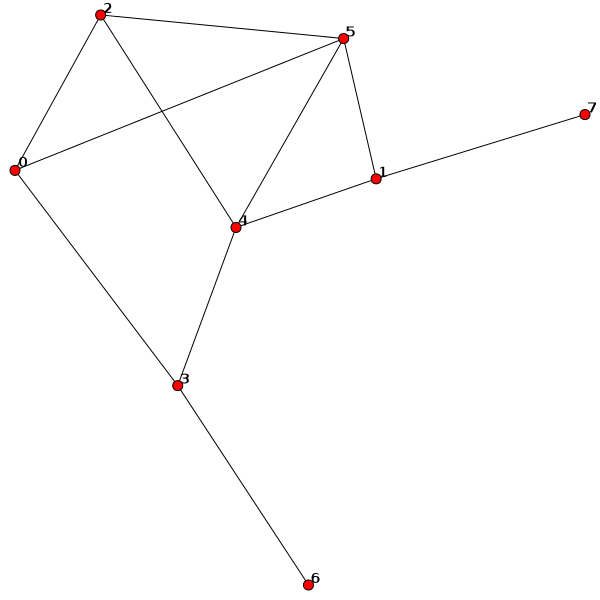
\includegraphics[width=0.6\textwidth]{preBFS}
  \caption{Esempio di un grafo indiretto non pesato}
  \label{fig:preBFS}
\end{figure}


\begin{figure}[H]
  \begin{algorithmic}
    \For {v $\in$ V} 
    \Comment {Inizializzazione: non conosciamo nessun
      cammino da $s$ a $v$} \State{v.d = $\infty$} \State{v.p = v}
    \EndFor
    \State{s.d = 0} \Comment {Inizializzazione: $s$ dista $0$ da s\`e
      stesso} \State{q = Queue()} \State{q.push(s)} \While{ !
      q.empty()} \State{v = q.pop()} \For{u $\in$ v.neigh} \If{u.d =
      $\infty$} \Comment{Cioè \`e la prima volta che raggiungiamo $u$}
    \State{u.d = v.d + 1} \State{u.p = v} \State{q.push(u)}
    \EndIf
    \EndFor
    \EndWhile
  \end{algorithmic}
%  \caption{Pseudocodice per la BFS}
\label{fig:BFScode}
\end{figure}
Non dimostreremo che questo algoritmo \`e corretto. L'idea che sta
alla base della dimostrazione \`e che i nodi vengono esaminati in
ordine di distanza non decrecente.

Osserivamo che l'algoritmo termina in $O\pa{M}$, infatti ogni nodo
viene inserito ed estratto dalla coda esattamente una volta e ogni
arco viene visitato una volta durante la visita del nodo di partenza.

\begin{figure}[h]
  \centering
  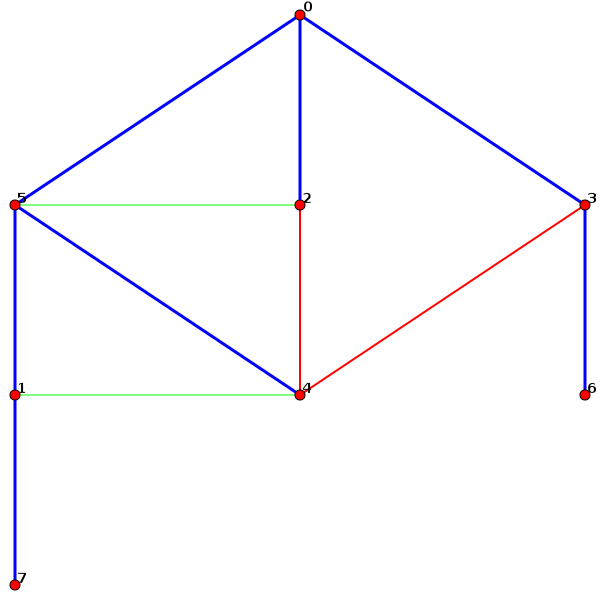
\includegraphics[width=0.6\textwidth]{BFS}
  \caption{Il grafo precedente dopo aver applicato una BFS con
    sorgente $0$, in blu gli archi scelti per l'albero, in rosso gli
    archi non scelti ma comunque appartenenti al DAG dei cammini
    minimi, in verde gli archi non appartenenti a cammini minimimi}
  \label{fig:BFS}
\end{figure}

I cammini minimi possono essere estratti in modo ricorsivo:
\begin{itemize}
\item \textbf{Caso base:} il cammino minimo da $s$ a $s$ \`e $(s)$.
\item \textbf{Passo induttivo:} un cammino minimo da $s$ a $v$ \`e
  $\tilde p + (v)$ dove $\tilde p$ \`e un cammino minimo da $s$ a $v.p$.
\end{itemize}

\subsection{Archi pesati: Dijkstra}

Nel caso in cui gli archi non abbiano tutti lunghezza unitaria, ma
comunque non negativa, dobbiamo usare l'algoritmo di Dijkstra
(introdotto in \cite{dijkstra}).

\begin{figure}[H]
  \begin{algorithmic}
    \For {v $\in$ V} 
    \Comment{Inizializzazione: non conosciamo nessun cammino da $s$ a
      $v$}
    \State{v.d = $\infty$} \State{v.p = v}
    \EndFor
    \State{S = $\emptyset$} \State{s.d = 0} \State{q =
      PriorityQueue()} \State{q.push(s,s.d)} \While{ ! q.empty()}
    \State{v = q.extract\_min()} \State{S = S $\cup$ \{v\}}
    \Comment{Sappiamo che abbiamo trovato la distanza esatta di $v$}
    \For{u $\in$ v.neigh} \If{u.d > v.d + w((v,u))} \Comment{Possiamo
      migliorare la distanza di $u$}\State{u.d = v.d + 1}
    \State{u.p = v} \State{q.push(u,u.d)} \Comment{Aggiorniamo $u$
      nella coda}
    \EndIf
    \EndFor
    \EndWhile
  \end{algorithmic}
%\caption{Pseudocodice per Dijkstra}
\end{figure}
L'idea che sta alla base di questo algoritmo \`e di trovare dei
cammini (non necessariamente minimi) da $s$ ad ogni vertice e
aggiornarli nel tempo. Manteniamo in una PriorityQueue tutti i
nodi di cui non consciamo ancora la loro distanza esatta ordinati per
la distanza ``temporanea'', ad ogni iterazione possiamo dire di
conoscere la distanza esatta del nodo nella coda con distanza pi\`u
bassa, infatti ogni cammino passante per un altro nodo nella coda non
potr\`a fare di meglio.


Anche questa volta possiamo disegnare l'albero dei cammini minimi con
la stessa procedura usata per il caso della BFS.

Per la complessit\`a vediamo che ogni arco viene visitato esattamente
una volta e, per ogni visita, viene effettuato un inserimento nella
PriorityQueue. Il numero di estrazioni dalla struttura di dati
PriorityQueue \`e maggiorato dal numero di inserimenti, quindi la
complessit\`a dell'algoritmo di Dijkstra \`e $O(M\log N)$ utilizzando
una coda di priorit\`a implementata con un min-heap.

\begin{figure}[h]
  \centering
  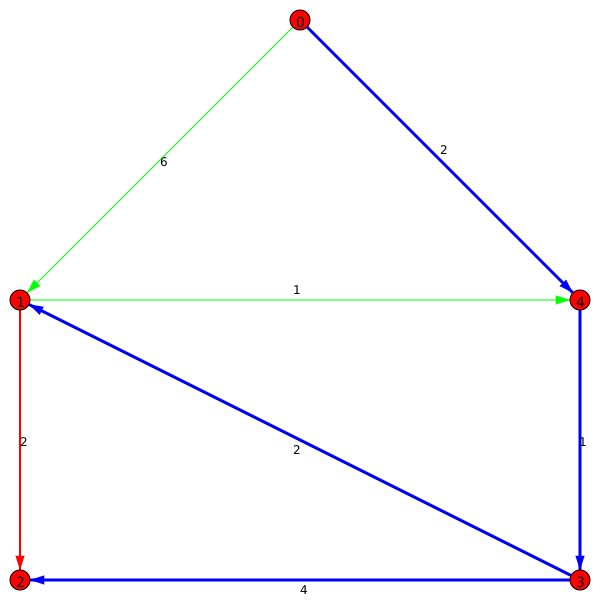
\includegraphics[width=0.6\textwidth]{dijkstra}
  \caption{Un grafo diretto pesato a cui è stato applicato Dijkstra
    con sorgente $0$, in blu gli archi scelti per l'albero, in rosso gli
    archi non scelti ma comunque appartenenti al DAG dei cammini
    minimi, in verde gli archi non appartenenti a cammini minimimi}
  \label{fig:dijkstra}
\end{figure}


\section{Cammini minimi fra ogni coppia}

Abbiamo visto che siamo in grado, data una sorgente $s\in V$, di
trovare tutti i cammini minimi da $s$ ad ogni nodo $v\in V$ e di
salvarci le distanze di ogni nodo dalla sorgente fissata. Ripetendo
questo procedimento al variare di $s\in V$ otteniamo questa
informazione per ogni coppia di nodi $(u,v)$ del grafo.

Nel nostro caso (archi di peso non negativo) possiamo applicare
l'algoritmo di Dijkstra su ogni nodo ottenendo un tempo di $O(NM\log
N)$ operazioni aritmetiche.

Ci chiediamo se esiste un metodo più veloce per estrarre alcune di
queste informazioni, possiamo sperare di riuscire a fare di meglio
evitando di fissare la sorgente.

Gli algoritmi che vedremo utilizzano la matrice di adiacenza del
grafo. Supponendo di aver numerato i nodi da $0$ a $N-1$, definiamo la
matrice di adiacenza di $G$ come la matrice $W$ con elementi
\[
  w_{i,j} = \left\{
    \begin{matrix}
      0 & \text{se } i = j \\
      w\pa{i,j} & \text{se } i\neq j,\; (i,j) \in E \\
      \infty & \text{se } i\neq j,\; (i,j) \not\in E
    \end{matrix}
  \right.
\]

Avendo supposto archi di peso non negativo, questa matrice avrà
elementi non negativi, inoltre se il grafo è indiretto questa matrice
diventa simmetrica.

\subsection{Tabella delle distanze}

Vogliamo calcolare la matrice delle distanze $D$ che ha per elementi
$d_{i,j} = \delta(i,j)$.

Consideriamo la matrice $L^{(m)}$ dove $l^{(m)}_{i,j}$ è il minimo
peso di un cammino da $i$ a $j$ che utilizzi al più $m$ archi. Siccome
un cammino tocca ogni nodo del grafo al pi\`u una
volta\footnote{Ricordiamoci che scegliamo cammini minimi aciclici} \`e
evidente che $L^{(N-1)} = D$, quindi cerchiamo un metodo induttivo per
calcolare $L^{(m)}$.

\textbf{Caso base:} per $m=0$ allora si ha
\[ l^{(0)} _{i,j} = \left\{
  \begin{matrix}
    0 & \text{se } i = j\\
    \infty & \text{se } i \neq j
  \end{matrix}
  \right.
\]

\textbf{Passo induttivo:} supponiamo di conoscere $L^{(m-1)}$, un
cammino con al più $m$ archi da $i$ a $j$ può avere:
\begin{itemize}
\item $m-1$ archi, quindi avrà lunghezza minima $l^{(m-1)}
  _{i,j}$ da cui $l^{(m)}_{i,j} \le l^{(m-1)} _{i,j}$
\item $m$ archi, allora lo possiamo spezzare come un cammino di
  $m-1$ archi (che arriverà ad un nodo che chiamiamo $k$) più un
  cammino di $1$ arco di lunghezza $w\pa{k,j}$. Per questo possiamo
  scrivere 
  \[ \forall k \in V\;\;\; l^{(m)}_{i,j} \le l^{(m-1)} _{i,k} + w\pa{
    k,j } \]
\end{itemize}
Quindi possiamo scrivere
\[ l^{(m)}_{i,j} = \min\set{ l^{(m-1)} _{i,j} , \min _{0\le k\le N-1}
  \set{ l^{(m-1)} _{i,k} + w\pa{k,j}} } = \min _{0\le k\le N-1} \set{
  l^{(m-1)} _{i,k} + w_{k,j}} \]
dove l'ultima uguaglianza possiamo scriverela perché abbiamo definito
gli elementi di $W$ come $w_{i,j} = w\pa{i,j}$ e abbiamo imposto
$w_{i,i} = 0$.

Implementando questa procedura impieghiamo $O(N)$ per calcolare un
$l^{(m)}_{i,j}$, $O(N^2)$ per calcolare tutta la matrice $L^{(m)}$ da
cui $O(N^4)$ per risolvere il problema. Questo tempo è superiore a
quello ottenuto applicando l'algoritmo di Dijkstra per ogni sorgente,
infatti abbiamo osservato che con quel metodo si impiegano $O(NM\log
N) = O( N^3 \log (N) )$ operazioni aritmetiche.

Vediamo come, leggendo l'aggiornamento della matrice $L$ come un
prodotto fra matrici, possiamo migliorare le prestazioni
dell'algoritmo. Ricordiamo che le entrate del prodotto fra matrici
possono essere scritte come
\[ c_{i,j} = \sum _k a_{i,k} \cdot b_{k,j} \] quindi considerando
$\mathbb{R}\cup \set{+\infty}$ con le operazioni di $\min$ e $+$
(rispettivamente al posto di $+$ e $\cdot$) otteniamo che
\[ L^{(m)} = L^{(m-1)} * W \]
dove $*$ è il prodotto di matrici con le nuove operazioni.

Lo spazio $\pa{\mathbb{R}\cup \set{+\infty} ,\min,+}$ ha le seguenti
propietà:
\begin{itemize}
\item $\min$ è associativa
\item $\min$ ha elemento neutro $\infty$
\item $\min$ è commutativa
\item $+$ è associativa
\item $+$ ha elemento neutro $0$
\item $+$ è commutativa
\item $+$ è distributiva rispetto a $\min$ (sia a destra che a sinistra)
\end{itemize}
In particolare osserviamo che $\min$ \emph{non} ammette inverso,
quindi il nostro spazio non \`e un anello.


Possiamo scrivere
\begin{align*}
  L^{(1)} & = & L^{(0)} * W & = & W \\
  L^{(2)} & = & L^{(1)} * W & = & W^2 \\
  & & \vdots & & \\
  L^{(N-1)} & = & L^{(N-2)} * W & = & W^{N-1} 
\end{align*}

Allora, visto che non siamo interessati alle matrici intermedie, ma
solo a $L^{(N-1)}$, possiamo calcolare induttivamente $W^{2^k}$ con la
formula
\[ W ^{2^k} = \pa{W ^{2^{k-1}}} ^2 \]
osservando che $L^{(m)} = L^{(N-1)}$ per $m \ge N-1$ si ha
\[ L^{(N-1)} = W^{2 ^{\ceil {\log \pa{ N-1} } } } \]

Siamo riusciti, in questo modo, a ridurre il tempo a $O\pa{ N^3 \log
  (N)}$
simile a quello di Dijkstra nel caso di grafo denso.

Potremmo pensare di migliorare questo metodo utilizzando la
moltiplicazione veloce fra matrici che impiega $O\pa{pN^\omega}$ tempo
dove $p$ è il tempo di un prodotto fra due entrate, $N$ la dimensione
della matrice e $2 \le \omega <3$ un esponente legato al metodo ottimo
(il cui valore \`e tuttora un problema aperto). In questo caso, però,
non lo possiamo applicare direttamente perché abbiamo osservato che la
struttura di $\pa{ \mathbb{R} \cup \set{\infty}, \min , +}$ non è un
anello e algoritmi come quello di Strassen utilizzando l'inverso della
prima operazione.

Tuttavia nel caso in cui le matrici siano ad entrate intere \`e
possibile procedere nel seguente modo: supponiamo che le matrici $A,B$
abbiano coefficienti in $\set{0, 1,...,k}$, allora scriviamo le
matrici $A'$ e $B'$ con coefficienti
\[ a'_{i,j} = x ^{a_{i,j}} \;\;\; b'_{i,j} = x ^{b_{i,j}} \]
dove $x$ è un'indeterminata. Sia quindi
\[ C' = A' \cdot B' \]
Dove stiamo usando il prodotto fra matrici, ma con coefficienti
nell'anello dei polinomi. Possiamo ottenere una martice $C$ i cui
coefficienti sono
\[ c _{i,j} = \mathrm{first}\pa{c'_{i,j}} \]
dove $\mathrm{first}$ ritorna il grado del monomio di grado più
piccolo in $c'_{i,j}$.

È facile convincersi che $C = A * B$, infatti 
\[ c'_{i,j} = \sum _k x^{a_{i,k} + b_{k,j}} \Rightarrow c_{i,j} =
\mathrm{first} \pa{c'_{i,j}} = \min _k \set{ a_{i,k} + b_{k,j} } \]

Quindi, nel caso di archi di lunghezza intera, siamo in grado di fare
il prodotto fra le matrici $L^{(i)}$ in $O\pa{pN^\omega }$ tempo dove $p$ è
il costo di un prodotto fra polinomi. Si pu\`o scrivere $p = O\pa{d
  \log d}$ dove $d$ \`e il diametro del grafo da cui otteniamo che
questo algoritmo utilizza $O\pa{ d N ^\omega \log d \log N}$
operazioni aritmetiche. Quindi, nel caso di grafi con diametri
piccoli ($d = \log\pa{N}$), come possono essere le reti sociali, abbiamo
migliorato le prestazioni del prodotto.

In \cite{funnymult} viene analizzato questo particolare prodotto tra
matrici proveniente da problemi di ricerca dei cammini minimi.


Esistono altri algoritmi per calcolare la tabella delle distanze. Per
esempio, l'algoritmo di Floyd–Warshall calcola la tabella delle
distanze (per un grafo senza cicli negativi) in $\Theta\pa{ N^3}$.
Citiamo anche il risultato di \cite{apspfmp}: possiamo calcolare la
tabella delle distanze di un grafo con archi di peso intero positivo
in $\tilde O\pa{ kN^\omega}$ tempo dove $k$ è la massima lunghezza di
un arco utilizzando, ancora una volta, il prodotto veloce tra matrici.

\subsection{I cammini minimi}

Ora che sappiamo calcolare le distanze tra due nodi del grafo,
possiamo concentrarci sull'estrarre i cammini minimi. Vale il seguente
lemma:
\begin{mylem}
  \label{lem:vicinibuoni}
  Dati $u,v \in V$ e $u'$ vicino di $u$ si ha che esiste un cammino
  minimo che utilizza l'arco $(u,u')$ se e solo se
  \[ \delta \pa{ u,v} = w\pa{ (u,u') } + \delta \pa{ u',v} \]
\end{mylem}

Grazie a questo lemma possiamo costruire ricorsivamente i cammini
minimi. Supponendo di essere interessati ai cammini minimi da $u$ a
$v$, se ne vogliamo trovare solo uno ci basta scegliere un vicino $u'$
``buono'' (cioè che rispetta l'uguaglianza del lemma
\ref{lem:vicinibuoni}) di $u$ e poi, ricorsivamente, proseguire
costruendo un cammino minimo da $u'$ a $v$. Se invece siamo
interessati a conoscere tutti i cammini minimi allora dobbiamo
calcolarci i cammini minimi per \emph{tutti} i vicini ``buoni'' di
$u$.

Il numero di cammini minimi tra due vertici può essere esponenziale
come si vede in questo semplice esempio:

\begin{figure}[H]
  \centering
  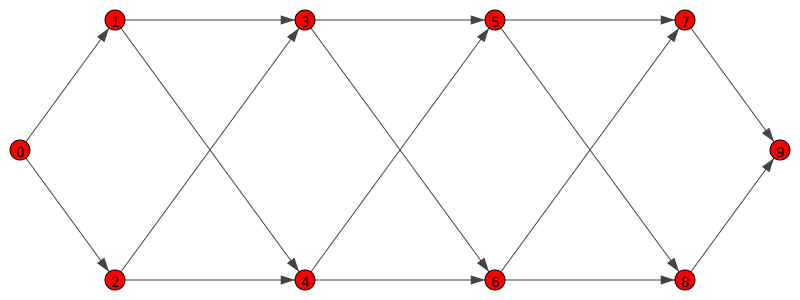
\includegraphics[width=0.7\textwidth]{diamantecatena}
  \caption{In questo esempio di grafo diretto non pesato vediamo che
    esistono esponenziali cammini minimi da $0$ a $9$}
  \label{fig:diamantecatena}
\end{figure}

Vedremo nel capitolo \ref{chap:oracolotutticammini} come salvare
queste informazioni in modo efficiente.

\section{Problema dei $k$ cammini più brevi}
\label{sec:kcammini}

Una generalizzazione del problema dei cammini minimi è il problema dei
$k$ cammini più brevi, cioè dati due vertici $u,v \in V$, ordinati i
cammini in $P(u,v)$ per lunghezza crescente, vogliamo estrarre i primi
$k$ cammini nell'ordine.

In questo caso potremmo dover considerare nuovamente cammini
contenenti cicli, infatti questi (pur non essendo minimi) potrebbero
comparire fra i $k$ cammini più brevi.

Questo problema è molto studiato in letteratura e noi non lo
tratteremo, citeremo solo alcuni risultati noti.

In \cite{kshortest} vengono forniti algoritmi su grafi diretti per
trovare:
\begin{itemize}
\item dati $u,v \in V$ trovare i primi $k$ cammini più brevi in
  $P\pa{u,v}$ in tempo $O\pa{m + n\log n + k}$;
\item una struttura (costruita in $O\pa{m+n\log n}$ tempo) che dati
  $u,v\in V$ ritorna in ordine di lunghezza i cammini in $P(u,v)$
  estraendo l'$i$-esimo in $O\pa{\log i}$ tempo;
\item dato $s\in V$ trovare i $k$ cammini più brevi per tutte le
  destinazioni $v\in V$ in $O\pa{m + n\log n + kn}$ tempo.
\end{itemize}

Uno dei problemi di questi algoritmi è che devono elaborare tutto il
grafo (che potrebbe essere molto grande) per poter restituire i primi
$k$ cammini minimi. Invece in \cite{kspheur} viene presentato
algoritmo che trova i $k$ cammini più brevi esplorando il grafo
\textit{on-the-fly}, utilizzando delle euristiche per migliorarne le
prestazioni ma ottenendo comunque, al caso pessimo, lo stesso tempo
dell'algoritmo di Eppstein cioè $O\pa{m + n\log n + k}$ tempo.

\chapter{Oracoli per distanze}
\label{chap:distanze}

Abbiamo visto come calcolare la tabella delle distanze, ora ci poniamo
il problema di salvarle. Il metodo banale di farlo (salvare la matrice
delle distanze $D$) richiede $O\pa{ N^2 \log d}$ bit dove $d$ è il
diametro del grafo ($d = O\pa{N}$ nel caso non pesato).

Diciamo che un certo algoritmo \`e un oracolo se \`e in grado di
rispondere alle nostre richieste (nel nostro caso la distanza tra due
punti qualsiasi) in tempo proporzionale all'output (nel nostro caso
$O\pa{1}$). In realt\`a saremo anche interessati ad algoritmi che
hanno tempi di risposta pi\`u lunghi ma comunque migliori rispetto al
metodo banale (per esempio logaritmici).

\`E naturale porsi due probelmi:
\begin{itemize}
\item è possibile salvarsi una struttura dati pi\`u piccola ($o
  \pa{ N^2}$) in modo da poter dare ancora una buona approssimazione
  della distanza tra due vertici? Vedremo questo problema nella
  sezione \ref{sec:oracoliapprossimati}
\item qual'\`e la struttura dati pi\`u piccola che contiene le
  informazioni esatte sulle distanza di un grafo e ammette
  interrogazioni in tempo costante? Vedremo questo nella
  sezione \ref{sec:oracoliesatti}
\end{itemize}

In questo capitolo useremo grafi non pesati, \`e comunque studiato
anche il caso pesato ma noi lo tralasceremo per semplicit\`a.

\section{Oracoli approssimati}
\label{sec:oracoliapprossimati}

In questa sezione ci poniamo il problema di usare poco spazio in
memoria pur continuando a saper stimare (ma senza pretendere di
restituire il valore esatto) la distanza fra due punti in un grafo.

Ricordiamo che salvare il grafo completo richiede $O\pa{ N + M }$
spazio che diventa $O\pa{ N^2}$ per grafi densi. Per questo dobbiamo
cercare degli approci alternativi.

\begin{mydef}[$r$-approssimazione]
  Diciamo che un certo algoritmo ritorna una $r$-approsimazione della
  distanza tra due punti se per ogni $u,v \in V$, detta $d(u,v)$ la
  distanza ritornata dall'algoritmo, si ha che
  \[ d\pa{u,v} \le r \delta\pa{u,v} \]
\end{mydef}

\subsection{Graph spanners}

Un metodo molto usato (introdotto in \cite{graphspanners}) consiste
nel salvare (e poi eventualmente preelaborare) un $t$-spanner del
grafo.

\begin{mydef}[$t$-spanner]
  Dato $G = (V,E)$ grafo diciamo che $G' = (V, E')$ \`e un $t$-spanner
  di $G$ se $E' \subseteq E$ e
  \[ \forall u,v \in V \;\; \delta _{G'} \pa{ u,v} \le t \delta _{G}
    \pa{ u,v} \]
  cio\`e la distanza di $G'$ \`e una $t$-approsimazione della distanza
  in $G$.
\end{mydef}

Se quindi troviamo un grafo $G'$ con $o\pa{ N^2}$ archi (per esempio
$O(N)$) con questa propriet\`a allora occupiamo $o(N^2)$
spazio per salvarlo e sappiamo rispondere ad una query di distanza in
$O(M)$ (il tempo di eseguire una BFS).

Possiamo caratterizzare un $t$-spanner anche con
\begin{mylem}
  $G' = (V,E')$ con $E' \subseteq E$ \`e un $t$-spanner per $G$ se
  \[ \forall (u,v) \in E\;\; \delta_{G'} (u,v) \le t \]
\end{mylem}
\begin{proof}
  Dalla definizione di $t$ spanner otteniamo facilmente questa
  uguaglianza, per l'implicazione inversa osseriviamo che, dati $u,v
  \in V$, preso un cammino minimo $p \in P(u,v)$ otteniamo la
  disuguaglianza della definizione applicando la disuguaglianza del
  lemma per ogni arco in $p$
\end{proof}

Questo semplice risultato ci mostra che ci sono delle limitazioni
negli spanner che possiamo costruire
\begin{mypro}
  In un grafo indiretto $G = (V,E)$ sia $k$ la lunghezza minima di un
  ciclo non banale in $G$, allora se $G' = (V,E')$ \`e un $t$-spanner
  di $G$ con $t < k-1$ si ha $G = G'$
\end{mypro}
\begin{proof}
  Supponiamo per assurdo che esista $(u,v) \in E' \setminus E$,
  siccome
  \[ \delta_{G'} (u,v) \le t < n -1 \] 

  Si ha che esiste un cammino aciclico composto da $h$ archi di $E'$
  da $u$ a $v$ con $h<k-1$, allora ricordando che $(u,v) \not\in E'$
  si ha che se aggiungiamo $(v,u)$ al cammino otteniamo un ciclo di
  lunghezza $h+1 < k$ da cui l'assuro.
\end{proof}

Ci poniamo allora il problema di dire quando esistono dei $t$-spanner
di un grafo con un certo numero di archi, purtroppo si ha che (teorema
che non dimostriamo)
\begin{myteo}
  Dato un grafo $G = (V,E)$ e due numeri $t,m\ge 1$ il problema di
  determinare se esiste un $t$-spanner di $G$ con al pi\`u $m$ archi
  \`e NP-completo.
\end{myteo}

Nonostante questo teorema \`e possibile studiare il problema in modo
asintotico.

Sempre in \cite{graphspanners} vengono dati i seguenti risultati:

\begin{myteo}
  Dato un grafo di $N$ vertici $G$ e $1<k<N$ esiste (ed \`e
  costruibile in tempo polinomiale) un $(4\log _k N +1)$-spanner con
  al pi\`u $kN$ archi.
\end{myteo}

\begin{mycor}
  Dato un grafo di $N$ vertici $G$ esiste (ed \`e costruibile in tempo
  polinomiale) un $O\pa{\log N}$-spanner con $O(N)$ archi.
\end{mycor}

\begin{mycor}
  Dato un grafo di $N$ vertici $G$ e per ogni $r\ge 1$ esiste (ed \`e
  costruibile in tempo polinomiale) un $(4r+1)$-spanner con
  $O(N^{1+1/r})$ archi.
\end{mycor}


\subsection{Altri risultati}

Anche supponendo di avere un grafo con pochi archi (magari perch\'e è
un $t$-spanner), potremmo non poterci permettere di elaborarlo ad ogni
richiesta di distanza, per questo sono stati sviluppati algoritmi che,
dopo una preelaborazione, salvano le informazioni sulle distanze in
poco ($o(N^2)$) spazio e permettono di ricavare la distanza
approssimata tra due punti in tempo costante.

In \cite{appdistoracl} gli autori presentano questo risultato:
\begin{myteo}
  Sia $G = (V,E)$ un grafo indiretto pesato con archi di peso non
  negativo e sia $k\ge 1$ intero, allora $G$ pu\`o essere
  preprocessato in $O\pa{kMN^{1/k}}$ tempo producendo una struttura
  dati occupante $O\pa{kN^{1+1/k}}$ spazio tale che in $O\pa{k}$ tempo
  \`e possibile tornare la distanza fra due punti approssimata di un
  fattore $2k-1$
\end{myteo}
\begin{mycor}
  Nelle ipotesi del teorema precedente fissando $k=2$ otteniamo che
  preprocessando il grafo in $O\pa{MN^{1/2}}$ si ottiene una struttura
  occupante $O\pa{N^{3/2}}$ che resituisce in $O\pa{1}$ la distanza
  tra sue punti approssimata di un fattore $3$
\end{mycor}
\begin{mycor}
  Nelle ipotesi del teorema precedente fissando $k=\floor{\log N}$ ottieniamo
  che che preprocessando il grafo in $O\pa{M\log N}$ si ottiene una
  struttura occupante $O\pa{N\log{N}}$ che resituisce in $O\pa{\log N}$ la
  distanza tra sue punti approssimata di un fattore $\log N$
\end{mycor}

In \cite{appdistoraclplus} viene migliorato questo risultato per
quanto riguarda il tempo di preelaborazione al costo di aggiungere un
fattore additivo all'errore di approssimazione della distanza.

Viene dato un primo risultato per grafi non pesati:
\begin{myteo}
  Sia $G = (V,E)$ un grafo indiretto non pesato e $k\ge 3$ un intero,
  allora \`e possibile costruire in $O\pa{ M + kN^{3/2 + 1/(2k) +
      1/\pa{2k-2}}}$ tempo una struttura dati occupate
  $O\pa{kN^{1+1/k}}$ spazio tale che dati $u,v\in V$ in $O\pa{k}$
  tempo sia possibile ritornare una distanza $\tilde \delta\pa{u,v}$
  tale che
  \[ \tilde \delta \pa{ u,v} \le \pa{2k -1}\delta\pa{ u,v} + 2 \]
\end{myteo}

Per grafi pesati con pesi interi non negativi vale un teorema simile
in cui l'errore additivo sulla distanza invece di essere $2$ diventa
$2 \max _{e\in E} w(e)$

\section{Oracoli esatti}
\label{sec:oracoliesatti}

Concentriamoci, per semplicit\`a, al caso di grafi indiretti con archi
non pesati. In questa sezione presenteremo il risultato proposto in
\cite{compactdistance}.

Ci chiediamo di poter rispondere in tempo costante a richieste di
distanza tra due punti qualsiasi del grafo ritornando la distanza
esatta. Vedremo nella sottosezione \ref{sec:oracoloesattoottimale} che
una struttura dati che soddisifi questa richiesta non pu\`o rompere la
barriera dei $\Omega\pa{ N^2}$ bit, attualmente noi lo sappiamo fare
in $O\pa{N^2 \log\pa{ N}}$, quindi possiamo migliorare.


\subsection{Risoluzione tramite etichettatura di un albero di ricoprimento}

Consideriamo un qualsiasi albero di ricoprimento di $G$ dove chiamiamo
$r$ la sua radice. Per ogni nodo $u\in V$ chiamiamo $f(u)$ il padre
nell'albero scelto e definiamo induttivamente $f^i(u) =
f\pa{f^{i-1}(u)}$ (poniamo $f^0(u)=u$).

\subsubsection{L'albero etichettato}

Scegliamo una sorgente $s\in V$ e consideriamo le distanze dei vertici
del grafo da $s$, per ogni nodo $u\in V$ definiamo la quantit\`a
\[ l_s (u) = \delta\pa{ u,s } - \delta\pa{ f(u),s} \]

Si ha il seguente lemma:
\begin{mylem}
  \[ \delta\pa{ u,s} = \delta\pa{ r,s} + \sum _{v\in \pi (u)\setminus
    \set{r}} l_s(v) \] dove $\pi (u)$ \`e il cammino nell'albero da
  $r$ a $u$.
\end{mylem}
\begin{proof}
  \begin{align*}
    &\delta\pa{ r,s} + \sum _{v\in \pi (u)\setminus \set{r}} l_s(v) =\\
    =& \delta\pa{ r,s} + \sum _{v\in \pi (u)\setminus \set{r}} \bra{
      \delta\pa{ v,s } - \delta\pa{ f(v),s} } =\\
    = & \delta\pa{ r,s} + \delta\pa{ u,s} - \delta\pa{ r,s}=\\
    = & \delta\pa{ u,s}
  \end{align*}
  Infatti la sommatoria \`e telescopica e si semplifica.
\end{proof}

Quindi ci basta salvare, al variare di $s\in V$, la quantit\`a
$\delta\pa{ r,s}$ e il vettore~ $l_s$. Poniamo, per semplicit\`a,
$l_s(r) = 0$ in modo da poter includere $l_s(r)$ nella sommatoria.

Abbiamo osservato che la distanza tra due nodi rispetta la propriet\`a
triangolare, da questa ricaviamo che 
\[ \abs { \delta\pa{ u,v} - \delta\pa{ w,v}} \le \delta\pa{ u,w} \]
specializzandola nel caso $w = f(u)$ e $v = s$
\[ l_s (u) = \delta\pa{ u,s} - \delta\pa{ f(u),s} \in \set{ -1, 0 ,
  1} \]

Quindi le nostre etichette sono ternarie, cio\`e possono assumere solo
tre valori.

\subsubsection{Dalle somme sui percorsi alle somme sui prefissi}

Visto che cerchiamo un modo per ottenere risposte in tempo costante,
non possiamo permetterci di calcolare la sommatoria ad ogni richiesta,
per questo vogliamo precalcolare in qualche modo queste sommatorie sui
percorsi.

Ci proponiamo ora di ricondurci ad un problema pi\`u studiato: le
sommatorie sui prefissi, cio\`e ci riconduciamo a calcolare la somma
dei primi elementi di una sequenza.

Data un'etichettatura $l$ su un albero $T$ costruiamo ricorsivamente
la seguente sequenza $L_T$
\begin{itemize}
\item \textbf{caso base:} se $T$ \`e vuoto allora $L_T = \bra{}$
\item \textbf{passo induttivo:} sia $T$ ha almeno un nodo e $u$ \`e la
  radice, siano $v_1,... ,v_k$ i figli di $u$ con $T_1,...,T_k$ i
  rispettivi sottoalberi, allora
  \[ L_T = \bra{ l(u) } + L_{T_1} + ... + L_{T_k} + \bra{ -l(u) } \]
\end{itemize}
Dove con $+$ intendiamo la concatenazione di sequenze. La sequenza
$L_T$ cos\`i definita avr\`a $2N$ elementi dove $N$ \`e la dimensione
di $T$.

Per capire meglio come \`e costruita la stringa $L_T$ pu\`o essere
utile vedere la figura~ \ref{fig:labeltree}.

\begin{figure}[h]
  \centering
  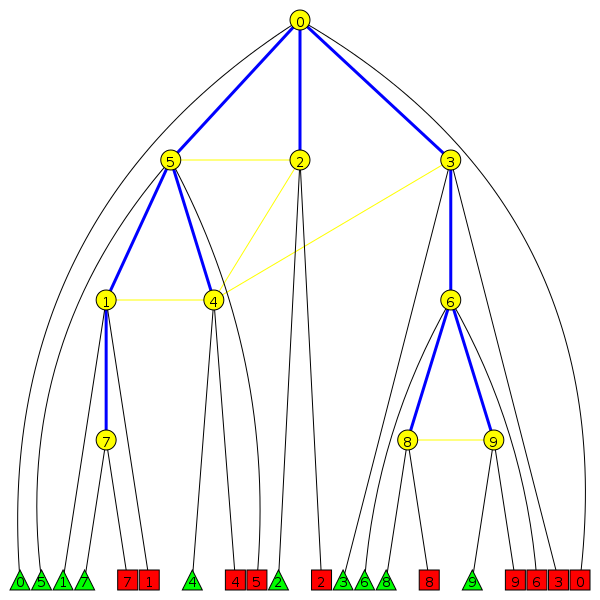
\includegraphics[width=1\textwidth]{labeltree}
  \caption{Un albero (nodi tondi gialli e archi blu) con riportate per
    ogni nodo $u$ le posizioni di $l(u)$ (triangoli verdi) e $-l(u)$
    (quadrati rossi) nella stringa associata all'albero. L'indice di
  $r_T(u)$ \`e dato dalla posizione nella stringa del triangolo
  associato ad $u$.}
  \label{fig:labeltree}
\end{figure}


Dato un nodo $u\in T$ chiamiamo $r_T(u)$ la posizione di $l(u)$ nella
stringa $L_T$, in questo modo \`e facile convincersi che 
\[ \sum _{v \in \pi(u)} l(v) = \sum _{i=0} ^
{r_T(u)} L_T[i] \]
infatti il valore di $l(v)$ per $v \not\in \pi(u)$ viene annullato da
$-l(v)$ scritto nella stringa nel momento in cui viene chiusa la
visita al sottoalbero di $v$, questo non accade per $v\in \pi(u)$
perch\'e la visita al suo sottoalbero (a cui appartiene $u$) non \`e
stata conclusa.

Osserviamo che $r_T$ non dipende da $l$ ma solo dalla struttura
dell'albero.

Ora abbiamo $\forall s\in V$ le etichette $l_s$ da cui possiamo
calcolare la corrispondente stringa (che chiameremo $L_s$), $r_T$
invece non dipende dall'etichettatura scelta ma solo dall'albero,
quindi ci basta salvarlo solo una volta.

\subsection{Somme prefisse precalcolate: Wavelet Tree}

Ci poniamo ora il problema di precalcolare e di salvare le somme
prefisse di una stringa $L$ fissata. Ricordiamoci che, essendo
l'etichettatura ternaria, gli elementi di $L$ sono solo~ $\set{-1, 0,
  1}$.

Ci vengono in aiuti i Wavelet Tree (struttura che non discuteremo nel
dettaglio) per i quali vale il seguente teorema:
\begin{myteo}
  Data una sequenza $S$ di $n$ caratteri presi dall'alfabeto $\Sigma$
  il Wavelet Tree costruito su $S$ occupa $nH_0(S) + o(n)$ bit e
  risponde alle seguenti richieste in $\log \abs{\Sigma}$ tempo:
  \begin{itemize}
  \item Ottieni il carattere $S[i]$
  \item $Rank_c (S,i)$: calcola il numero di occorenze del carattere~
    $c\in \Sigma$ nella stringa $S[0:i]$ (cio\`e nei primi~ $i+1$
    elementi di $S$)
  \item $Select _c (S,i)$: calcola la posizione dell'$i$-esima
    occorrenza di~ $c\in \Sigma$ in~ $S$
  \end{itemize}
\end{myteo}

Dove $H_0(S)$ \`e l'ordine $0$ dell'entropia empirica di $S$ che
possiamo definire (chiamando $n_\sigma$ il numero di occorenze del
carattere $\sigma\in \Sigma$ in $S$ e $n$ il numero totale di
caratteri in $S$) come:
\[ H_0(S) = - \sum _{\sigma \in \Sigma} \frac{n_\sigma}{n} \log \pa{
  \frac{n_\sigma}{n}} \] 

Dato che $H_0(S) \le \log \abs{\Sigma}$ possiamo scrivere che un
Wavelet Tree occupa al pi\`u $\log \abs{\Sigma} n + o(n)$ bit.

Tornando al nostro problema delle somme prefisse, possiamo ora
presentare il seguente risultato:
\begin{mypro}
  Salvando la stringa $L$ con un Wavelet Tree possiamo calcolare una
  somma prefissa
  \[ \sum _{i=0} ^ {k} L[i] = \sum _{\sigma \in \Sigma} \sigma Rank
  _\sigma (S,k) \] 
  in $O\pa{ \abs{\Sigma} \log \abs{\Sigma} }$ mantendendo una struttra
  dati occupante $n\log \abs{\Sigma} + o(n)$ bit.
\end{mypro}

Nel nostro caso $\Sigma = \set{ -1,0,1}$ e $n = 2N$, quindi in tempo
costante riusciamo a calcolare una somma prefissa utilizzando un
Wavelet Tree che occupa $2\log\pa{ 3} N + o(N)$ spazio.


\subsection{Complessit\`a e ottimalità}
\label{sec:oracoloesattoottimale}

Abbiamo gi\`a visto che siamo in grado di fare richieste di distanza
in tempo costante. Vediamo quanto stiamo spendendo in spazio.

Dobbiamo salvare:
\begin{itemize}
\item l'albero $T$ scelto occupando $O\pa{N\log\pa{N}}$ bit
\item le distanze $\delta\pa{s,r}$ al variare di $s\in V$ occupando
  $O\pa{ N \log N}$ bit in totale
\item il vettore $r_T$ occupando $O\pa{N \log\pa{N}}$ bit 
\item al variare di $s\in V$ il Wavelet Tree associato a $L_s$,
  utilizzando in tutto $2\log\pa{3} N^2 + o(N^2)$ bit
\end{itemize}
quindi stiamo utilizzando in tutto $2\log\pa{3} N^2 + o(N^2)$ bit.

Osserviamo che esiste una corrispondenza biunivoca fra grafi indiretti
non pesati e matrici distanza, in un grafo di $N$ nodi esitono
$\binom{N}{2} = \pa{N(N-1)}/{2} = N^2/2 + o(N^2)$ archi possibili,
quindi il numero di grafi possibili \`e $2^{N^2/2 + o(N^2)}$,
da cui il numero minimo di bit che deve usare il nostro oracolo sar\`a
\[ \log \pa{ 2^{N^2/2 + o(N^2)} } = \frac{N^2}{2} + o(N^2) \]

La nostra soluzione occupa $4 \log \pa{3}$ volte lo spazio dato dal
limite inferiore, possiamo guadagnare un fattore $2$ se salviamo solo
le distanze $\delta\pa{u,v}$ con $u<v$ (sfruttando la simmetria delle
distanze) abbassandoci a $2\log \pa{3}$.

\`E possibile, partizionando $T$ in macro-micro-alberi, abbassare lo
spazio utilizzato a $\pa{\log\pa{3} /2} N^2 + o(N^2)$ continuando ad
ammettere query in tempo costante, ma noi non lo vedremo.

\subsection{Possibile generalizzazione: archi pesati}

Per grafi indiretti pesati, il limite inferiore in spazio teorico
diventa $\Omega\pa{ N^2 \log k}$ bit (dove $k$ è il massimo modulo
della lunghezza di un arco). Partendo dalla struttura presentata per
archi non pesati \`e possibile ottenerne una che, pur supportando
query in tempo costante non dipendente da $k$, occupa il seguente
numero di bit:
\[ \frac{ \ceil { \log{2k+1} } }{2} N^2 + o(N^2) \]

\chapter{Oracolo per scrivere tutti i cammini minimi}
\label{chap:oracolotutticammini}

Discutiamo il problema di costruire un oracolo in grado di restituire,
data una coppia di vertici, \textbf{tutti} i cammini minimi aciclici
tra la coppia.

Per semplicit\`a supponiamo che gli archi abbiano lunghezza positiva
non nulla (in modo da non dover gestire i cicli di lunghezza
nulla). Il caso generale pu\`o essere ricondotto a questo collassando
i vertici collegati da archi di lunghezza nulla (nel caso non diretto)
o aggiungendo degli opportuni archi (nel caso diretto).

Ricordiamo che un oracolo deve impiegare, nell'elaborare una
richiesta, tempo proporzionale all'output. Quindi, in questo caso,
tempo proporzionale al numero di archi restituiti, vale a dire
\[ O\pa{ c(u,v) \delta (u,v) } \]
dove $c(u,v)$ \`e il numero di cammini minimi in $P(u,v)$

Ricordiamo che, come abbiamo visto nell'esempio della figura
\ref{fig:diamantecatena}, il numero di cammini tra una coppia di vertici
pu\`o essere esponenziale, quindi potremmo essere interessati anche a
poter chiedere solo un certo numero $k$ di cammini, cos\`i facendo ci
si avvicinerebbe al problema dei $k$ cammini pi\`u brevi trattato
nella sezione \ref{sec:kcammini}.

Nel caso particolare di $k=1$ (cio\`e ci basta conoscere un solo
cammino) abbiamo gi\`a osservato, come conseguenza del lemma
\ref{lem:vicinibuoni}, che ci basta salvare per ogni coppia di vertici
$u,v$ un vicino ``buono'' $u'$ di $u$, cio\`e tale che esiste un
cammino minimo da $u$ a $v$ che ha come secondo vertice $u'$. In
questo modo stiamo occupando $O\pa{N^2 \log N}$ bit di memoria e
rispondiamo alle richieste in $O\pa{ \delta\pa{u,v}}$, cio\`e il tempo
cercato.

\section{Un primo algoritmo}
\label{sec:camminibanale}

Siano $u,v$ due vertici tra i quali stiamo cercando tutti i cammini
minimi, siano essi $p_1,p_2,...,p_c$ con $c = c(u,v)$.

Siano $u_1,..., u_c$ i nodi che compaiono in seconda posizione nei
cammini (in prima compare $u$). Visto che, in generale, ci saranno
delle ripetizioni possiamo supporre (a meno di riordinare i $p_i$) che
esiste $n$ tale che $u_1,...,u_n$ sono tutti distinti e che ogni nodo
in $\set{ u_{n+1},..., u_c}$ sia la ripetizione di un qualche nodo
$\set{ u_1,..., u_n}$.

Possiamo allora partizionare l'insieme $\set{p_1,... ,p_c}$ in $n$
insiemi $P_1, ..., P_n$ tali che $p_i \in P_k$ se e solo se il secondo
vertice di $p_i$ \`e $u_k$.

Definiamo anche gli insiemi $\pa{ \tilde P_i} _{i=1,..,n}$ dove
$\tilde P_i$ contiene tutti i cammini di $P_i$ a cui \`e stato rimosso
il primo vertice $u$, ci\`o significa che $\tilde P _i \subseteq P\pa{
  u_i, v}$.

\begin{mypro}
  Per ogni $i \in \set{ 1,...,k}$ si ha che $\tilde P _i$ contiene
  tutti e soli i cammini minimi tra $u_i$ e $v$.
\end{mypro}
\begin{proof}
  Tutti questi sono cammini minimi, infatti sappiamo che un
  sottocammino di un cammino minimo \`e ancora minimo.

  D'altra parte se $q \in P(u_i,v)$ \`e un cammino minimo allora $(u)
  + q$ diventa un cammino minimo in $P(u,v)$ e quindi esiste $j \in
  \set{ 1,...,c}$ tale che $(u) +q = p_j$. Siccome il secondo vertice
  di $p_j$ \`e $u_i$ si ha che $p_j \in P_i$ e quindi $q \in \tilde P
  _i$.
\end{proof}

Questa proposizione ci dice che per conoscere i cammini minimi in
$P(u,v)$ ci basta conoscere i cammini minimi in $P(u_i,v)$ al variare
di $u_i \in \set{ u_1,..., u_n}$ dove $\set{ u_1,..., u_n}$ sono i
vicini ``buoni'' definiti dal lemma \ref{lem:vicinibuoni}.

Presentiamo quindi un primo algoritmo, molto semplice, per costruire
un oracolo in grado di ritornare tutti i cammini minimi.

\textbf{Preelaborazione:}
\begin{enumerate}
\item Calcola la matrice $D$ delle distanze fra ogni coppia di vertici;
\item per ogni coppia $u,v\in V$ cerca i vicini ``buoni'' di $u$
  verificando l'uguaglianza del lemma \ref{lem:vicinibuoni} e salvali.
\end{enumerate}

\textbf{Risposta ad una richiesta}
\begin{enumerate}
\item Siano $u,v$ i nodi di cui dobbiamo ritornare i cammini minimi;
\item carichiamo dalla memoria l'insieme $u_1,..., u_n$ dei vicini
  buoni di $u$;
\item per ogni $u_i$ calcoliamo l'insieme $\tilde P _i$ dei cammini
  minimi in $P(u_i,v)$;
\item sia $P_i = \set{ (u) + \tilde p _i \mid \tilde p_i \in \tilde
    P_i }$;
\item restituiamo $\bigcup _i P_i$
\end{enumerate}

Per la preelaborazione utilizziamo $O\pa{ NM}$ tempo, infatti per ogni
vertice di arrivo $v$ stiamo esaminando tutti gli archi uscenti da
ogni altro vertice, il risultato della preelaborazione occupa $O\pa{
  NM \log {N}}$ bit.

Si pu\`o dimostrare per induzione sulla distanza tra i nodi che una
richiesta viene elaborata in tempo proporzionale all'output, quindi
abbiamo scritto un oracolo.

Osserviamo che per grafi densi arriviamo ad occupare $O\pa{ N^3 \log
  \pa{N}}$ spazio.

\section{Un algoritmo con tempo di query non ottimale}

Abbiamo visto che con l'algoritmo precedente occupiamo, al caso
pessimo, $O\pa{ N^3 \log\pa{N}}$ bit, potremmo pensare di
diminuire lo spazio occupato calcolando i vicini buoni al momento
della richiesta.

Nella preelaborazione, quindi, rimane solo il calcolo della matrice
delle distanze e il suo salvataggio (che sappiamo fare in $\tilde
O\pa{ N^2}$ bit), ma nella procedura eseguita al momento richiesta
dobbiamo aggiungere la ricerca dei vicini ``buoni''.

La ricerca dei vicini buoni per un vertice utilizza tempo
proporzionale al suo grado, visto il carattere ricorsivo
dell'algoritmo proposto dovremo effettuare questa ricerca per ogni
vertice presente in un qualche percorso minimo. Possiamo dire che
esamineremo ogni arco al pi\`u due volte, per questo il tempo di
elaborazione di una richiesta diventa $O\pa{ c\pa{u,v} \delta\pa{u,v}
  + M}$. \`E possibile costruire esempi in cui questo peggiora il caso
precedente, per esempio potremmo avere un solo cammino minimo ma ci
troviamo a dover esaminare tutti gli archi del grafo. TODO: esempio
disegnino

Siamo riusciti a migliorare lo spazio occupato al costo di peggiorare
il tempo impiegato per elaborare una richiesta ottenendo, quindi, un
algoritmo che non \`e pi\`u un oracolo.

\section{Una classe particolare: grafi planari}

Vediamo come per i grafi planari si possa costruire un oracolo che, al
caso pessimo, occupa meno spazio rispetto all'oracolo presentato nella
sezione \ref{sec:camminibanale}.

\begin{mydef}[Grafo planare]
  Un grafo si dice \textit{planare} se pu\`o essere rappresentato in
  un piano in modo che gli archi non si intersechino se non sui
  vertici.
\end{mydef}

Si vede facilmente che un sottografo di un grafo planare \`e ancora
planare. 

Sfruttando la struttura dei grafi planari data dal \textit{separation
  theorem} riusciamo a migliorare lo spazio occupato dal nostro
oracolo pur mantenendo tempo di elaborazione proporzionale all'output.

\subsection{Separation theorem}

Per i grafi planari in \cite{separator} viene dimostrato il seguente
teorema
\begin{myteo}[\textit{Separation theorem}]
  Dato un grafo planare $G = (V,E)$, detto $N = \abs{V}$ \`e
  possibile partizionare $V$ in tre insiemi $A,B,S$ tali che
  \begin{itemize}
  \item $A$ e $B$ hanno al pi\`u $2n/3$ vertici ciascuno
  \item $S$ ha $O\pa{ \sqrt{N}}$ vertici
  \item non esistono archi tra $A$ e $B$
  \end{itemize}
\end{myteo}

Quindi questo teorema ci permette di dividere un grafo planare in due
sottografi (anch'essi planari) $A$ e $B$ separati dai nodi in $S$, per
questo possiamo applicare metodi di \textit{divide et impera} al
grafo.

Vediamo, per esempio, come ci viene in aiuto in un contesto di ricerca
di cammini minimi. Siano quindi $u,v \in V$, se dividiamo $V$ con il
separation theorem possiamo distinguere tre casi: 
\begin{enumerate}
\item $u \in A, v\in B$ (o viceversa): allora un cammino minimo in
  $P(u,v)$ deve passare attraverso un nodo in $S$, quindi ci siamo
  ricondotti a studiare i cammini minimi in $P(u,s)$ e $P(s,v)$ al
  variare di $s \in S$, da questi poi possiamo ricostruire i cammini
  minimi in $P(u,v)$;
\item $u,v \in A$ (o $B$): possiamo limitarci a studiare $A$ che \`e
  più piccolo di $V$;
\item $u\in s, v\in A$ (o $B$): consideriamo $A\cup \set{s}$ che \`e
  pi\`u piccolo di $V$.
\end{enumerate}
avendo osservato che $A$ e $B$ sono a loro volta planari, possiamo
riapplicare il \textit{separation theorem} al grafo ridotto e ripetere
il procedimento.

Osserviamo che, nel caso in cui volessimo precalcolare in modo
ricorsivo le scomposizioni, detta $A,B,S$ la partizione data dal
teorema ci conviene riapplicare il teorema agli insiemi $A\cup S$ e
$B\cup S$, infatti in questo modo assorbiamo anche il terzo caso.

La scomposizione ricorsiva ha, al pi\`u, profondit\`a $\log
_{\frac{2}{3}} \pa{N}$, cio\`e $O\pa{ \log\pa{N}}$.

\subsection{Un oracolo in spazio $\tilde O(n^{2.5})$}

Supponiamo di aver partizionato ricorsivamente il nostro grafo
utilizzando il \textit{separation theorem}, vogliamo costruire un
oracolo che sfrutti questa struttura.

Vista la caratterizzazione che abbiamo dato di un algoritmo
\textit{divide et impera}, discutiamo cosa deve fare l'oracolo nei tre
casi:
\begin{enumerate}
\item se $u,v$ stanno in due partizioni diverse del grafo dobbiamo
  ricondurci a studiare i cammini attraverso $S$, siccome non abbiamo
  tempo di controllare tutte le distanze siamo costretti a salvarci i
  nodi in $S$ che appartengono ad un qualche cammino minimo in
  $P(u,v)$.
\item se $u,v$ appartengono alla stessa partizione allora ci
  scendiamo nelle partizioni prescelte fino a trovare una partizione
  che li divida
\item il terzo caso, grazie alla scelta del partizionamento, \`e
  uguale al secondo
\end{enumerate}

Quindi per ogni coppia di vertici siamo interessati a sapere qual'\`e
la partizione che li separa e, in questa separazione, quali sono i
nodi separanti attraverso i quali passa un cammino minimo.

Siamo arrivati quindi a costuire il seguente algoritmo:

\textbf{Preelaborazione:}
\begin{enumerate}
\item Calcola la matrice delle distanze;
\item calcola in modo ricorsivo le partizioni di $V$;
\item per ogni coppia di vertici $u,v$ considera la partizione meno
  fine che li divide, sia $S$ l'insieme separatore;
\item salva l'insieme dei vertici $s\in S$ tali che $\delta\pa{u,s} =
  \delta\pa{s,v}$.
\end{enumerate}

\textbf{Risposta ad una richiesta:}
\begin{enumerate}
\item Siano $u,v$ i vertici di cui vogliamo calcolare i cammini minimi;
\item leggi dalla memoria l'insieme $\set{s_1,...,s_k}$ dei vertici che
  separano $u$ da $v$;
\item per ogni $s_i \in \set{s_1,...,s_k}$ calcola (per ricorsione) i
  cammini minimi in $P(u,s)$ e $P(s,v)$, sommando ogni possibile
  coppia di cammini otteniamo l'insieme $P_i$ di tutti i cammini
  minimi passanti per $s_i$;
\item se esiste un arco tra $u$ e $v$ ed \`e tale che $\delta\pa{ u,v}
  = w(u,v)$ aggiungi l'insieme~ $P_0 = \set{ (u,v) }$;
\item Ritorna $\bigcup _i P_i$.
\end{enumerate}

Il tempo di risposta \`e quello cercato, infatti per ogni $s_i$
elaborato esiste almeno un cammino minimo e, quindi, non stiamo
sprecando tempo.

Vediamo lo spazio occupato, per ogni coppia di nodi $u,v$ dobbiamo
salvarci l'insieme dei vertici separatori dai quali passa almeno un
cammino minimo, ma questi sono al pi\`u $O\pa{ \sqrt{N}}$ e, quindi,
stiamo occupando $O\pa{ N^{2.5} \log\pa{ N} }$ bit.

\section{Miglioriamo l'algoritmo}

Cerchiamo di migliorare l'algoritmo proposto alla sezione
\ref{sec:camminibanale}. Facendo alcune considerazioni sui cammini
minimi riusciamo a diminuire il numero di vicini da salvare senza
riuscire, per\`o, a diminuire lo spazio utilizzato nel caso pessimo.

Siano $u,v\in V$ i nodi di cui vogliamo trovare i cammini minimi.

Supponiamo di conoscere un vicino buono $u'$ di $u$ e di aver gi\`a
trovato, ricorsivamente, tutti i cammini minimi da $u'$ a $v$, abbiamo
quindi un insieme $W \subseteq V$ di vertici attraverso i quali passa
un qualche cammino minimo che abbiamo gi\`a trovato.

Sia $w \in W$, noi conosciamo tutti i cammini minimi da $u$ a $w$ che
hanno $u'$ come secondo vertice. In realt\`a a noi interessano tutti i
cammini minimi in $P(u,w)$, quindi possiamo scoprire nuovi cammini
minimi semplicemente cercando i cammini minimi in $P(u,w)$ e
concatenandoli con quelli in $P(w,v)$ (che gi\`a conosciamo).

In questo modo abbiamo ampliato l'insieme $W$ dei vertici usati da un
qualche cammino minimo in $P(u,v)$ e avremo, quindi, nuovi nodi $w\in
W$ su cui applicare il ragionamento precedente. Fra questi potrebbero
esserci anche nuovi vicini ``buoni'' che, quindi, non ci servir\`a
salvare.

Vediamo come verrebbe elaborata una richiesta di cammini:
\begin{enumerate}
\item Siano $u,v$ i nodi in input;
\item $P = \emptyset$ insieme dei cammini minimi che vogliamo costruire
\item $W = \emptyset$ l'insieme dei nodi da cui possiamo passare e non
  abbiamo ancora visitato;
\item $Z = \emptyset$ l'insieme dei nodi da cui possiamo passare e
  abbiamo gi\`a visitato;
\item sia $N$ l'insieme (ridotto) dei vicini ``buoni'' per raggiungere
  $v$ da $u$;
\item $W = W \cup N$;
\item per ogni $w \in W$
  \begin{enumerate}
  \item $Z = Z \cup \set{w}$;
  \item sia $P'$ l'insieme dei cammini minimi in $P(u,w)$;
  \item sia $P''$ l'insieme dei cammini minimi in $P(w,v)$;
  \item sia $W'$ l'insieme dei nodi toccati dai camminini in $P'$;
  \item sia $W''$ l'insieme dei nodi toccati dai camminini in $P''$;
  \item $P = P \cup \set{ p' + p'' \mid p' \in P' , \ p'' \in
      P''}$\footnote{In realtà sarebbe $p' - (w) + p''$ per evitare la
      ripetizione del nodo $w$ fra i due cammini, lo abbiamo
      tralasciato per semplicit\`a.};
  \item $W = W \cup \pa{ \pa{ W' \cup W'' } \setminus Z }$ salviamo i
    nuovi nodi scoperti;
  \end{enumerate}
\item resitituisci $P$.
\end{enumerate}

Vedremo nella prossima sezione che non siamo riusciti a migliorare lo
spazio occupato al caso pessimo.

\subsection{Struttura dei cammini minimi}

Questo algoritmo evidenzia una particolare struttura del grafo
(aciclico diretto) dei cammini minimi che ora analizziamo nel caso di
grafi indiretti.

Sia quindi $H = H(u,v) = (W,F)$ il sottografo di $G$ dei cammini
minimi fra $u$ e $v$. Questo \`e un sottografo del grafo dei cammini
minimi con sorgente in $u$, siccome quest'ultimo \`e un grafo aciclico
diretto (lo abbiamo dimostrato nella proposizione~ \ref{pro:DAG})
allora anche $H$ \`e un grafo aciclico diretto.

Sia $H' = (W',F')$ il sottografo di $H$ ottenuto con $W' = W \setminus
\set{u,v}$ e $F' = F \cap W' \times W'$, cio\`a abbiamo tolto gli
estremi $u,v$ da $H$ e stiamo considerando solo i nodi intermedi.

Il grafo $H$ \`e connesso\footnote{Qui usiamo una nozione debole di
  connessione, diciamo che un grafo diretto $G$ \`e connesso se lo \`e
  visto come un grafo indiretto} mentre, in generale, non lo sar\`a
$H'$. Siano quindi $H_1, ..., H_n$ le componenti connesse di $H$.

\begin{mypro}
  Dato $H_1$ connesso basta conoscere un solo vertice $h \in H_1$
  qualsiasi per poter conoscere tutto $H_1$ utilizzando il metodo
  descritto precedentemente.
\end{mypro}
\begin{proof}
  Sia $\tilde H \subseteq H_1$ l'insieme dei nodi che non vengono
  visitati, supponiamo per assurdo $\tilde H \neq \emptyset$. Siccome
  $H_1$ \`e connesso deve esistere un arco $f$ che collega $\tilde H$
  a $H_1 \setminus \tilde H$. Quest'arco ha un vertice in $H_1$ che
  chiamiamo $w$.

  Nella visita di $w$ abbiamo trovato, ricorsivamente, tutti i cammini
  minimi in $P(u,w)$ e in $P(w,v)$, in almeno uno di questi due
  insiemi (a seconda della direzione dell'arco) deve esserci un
  cammino che passa per $f$ (altrimenti $f\not\in F$), questo vuol
  dire che anche l'altro estremo di $f$ sta in $H_1 \setminus \tilde
  H$, ma $f$ l'abbiamo preso come un arco da $\tilde H$ a $H_1
  \setminus \tilde H$ da cui l'assurdo.
\end{proof}
\begin{mycor}
  Usando il nuovo algoritmo ci basta salvare un vicino ``buono'' per
  ogni componente connessa di $H$.
\end{mycor}

\section{Caso pessimo del nuovo algoritmo}
\label{sec:casopessimo}

Il caso in cui la nostra strategia precedente fallisce nel
diminuire lo spazio utilizzato \`e il seguente

\begin{figure}[H]
  \centering
  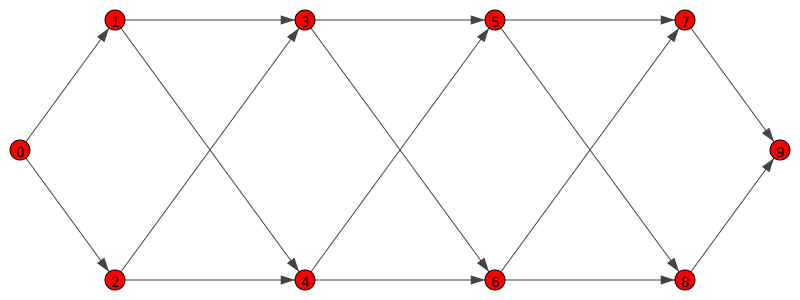
\includegraphics[width=0.9\textwidth]{diamante}
  \caption{Due nodi fra cui abbiamo una componente per ogni cammino}
  \label{fig:diamante}
\end{figure}


Viste le considerazioni che abbiamo fatti sulla struttura dei cammini
minimi, questo grafo riassume la struttura dei cammini minimi fra una
coppia di vertici. Possiamo immagginare, infatti, di aver collassato
ogni componente connessa ad un singolo nodo.

Questo esempio, pur raggiungendo il caso pessimo di spazio occupato,
sta ancora sotto la soglia di $O\pa{N^2}$ perch\'e il grafo \`e
sparso. Si pu\`o raggiungere il limite di $O\pa{ N M \log \pa{N} } =
O\pa{N^3 \log\pa{N}}$ bit considerando il seguente esempio:

\begin{figure}[H]
  \centering
  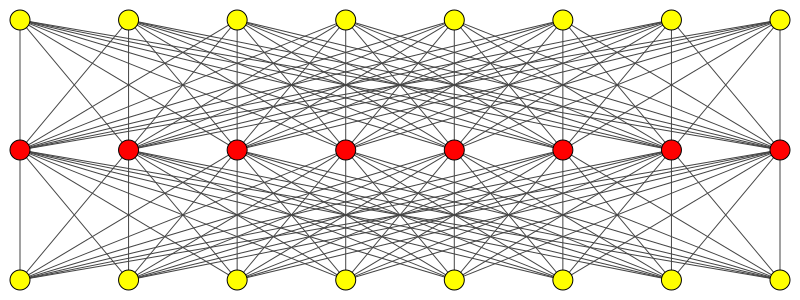
\includegraphics[width=1\textwidth]{diamantemultiplo}
  \caption{La struttura della figura \ref{fig:diamante} ripetuta in
    modo da ottenere il caso pessimo in un grafo denso}
  \label{fig:diamantemultiplo}
\end{figure}


\subsection{Un caso difficile}

Guidati dagli esempi visti, proponiamo alcune indicazioni su come
costruire un grafo ``difficile'' che ci possa dare un'indicazione
sullo spazio minimo che pu\`o utilizzare un oracolo per cammini
minimi.

Consideriamo un grafo indiretto non pesato bipartito $G = (V,E)$ i cui
vertici sono divisi in due insiemi di $N_1$ e $N_2$ nodi ciascuno,
cio\`e
\[ A = \set{a_1,....,a_{N_1} } ,\; B = \set{b_1,...,b_{N_2}} \;\;\; V =
A\cup B \]
tutti gli archi avranno estremi in due insiemi diversi, cio\`e
\[ E \subseteq A \times B \cup B \times A \]
sia $N = N_1 + N_2$ e $M = \abs{E}$.


Vogliamo costruire un grafo con queste caratteristiche che ogni
oracolo per cammini minimi richieda $\Omega \pa{ NM }$ spazio per
essere memorizzato, in mod da raggiungere (a meno di fattori
logaritmici) lo spazio richiesto dal nostro algoritmo.

Nell'analisi ci limiteremo ad analizzare i cammini minimi tra due nodi
in $A$ a distanza $2$. In particolare, viste le limitazioni su $E$, si
ha che i cammini minimi in $P(a,a')$ sono in corrispondenza biunivoca
con l'insieme
\[ \neigh(a) \cap \neigh(a') \subseteq B \]
dove $\neigh(u)$ indica i vicini del vertice $u$.

Rileggendo questa scrittura vediamo che quello che stiamo
effettivamente cercando \`e un oracolo per interesezioni di insiemi.






\bibliographystyle{alpha}
\bibliography{funnymult,apspfmp,kshortest,kspheur,graphspanners,appdistoracl,appdistoraclplus,compactdistance,separator,cormen,dijkstra}





\end{document}

